\documentclass[11pt]{article}

    \usepackage[breakable]{tcolorbox}
    \usepackage{parskip} % Stop auto-indenting (to mimic markdown behaviour)
    

    % Basic figure setup, for now with no caption control since it's done
    % automatically by Pandoc (which extracts ![](path) syntax from Markdown).
    \usepackage{graphicx}
    % Maintain compatibility with old templates. Remove in nbconvert 6.0
    \let\Oldincludegraphics\includegraphics
    % Ensure that by default, figures have no caption (until we provide a
    % proper Figure object with a Caption API and a way to capture that
    % in the conversion process - todo).
    \usepackage{caption}
    %\DeclareCaptionFormat{nocaption}{}
    %\captionsetup{format=nocaption,aboveskip=0pt,belowskip=0pt}

    \usepackage{float}
    \floatplacement{figure}{H} % forces figures to be placed at the correct location
    \usepackage{xcolor} % Allow colors to be defined
    \usepackage{enumerate} % Needed for markdown enumerations to work
    \usepackage{geometry} % Used to adjust the document margins
    \usepackage{amsmath} % Equations
    \usepackage{amssymb} % Equations
    \usepackage{textcomp} % defines textquotesingle
    % Hack from http://tex.stackexchange.com/a/47451/13684:
    \AtBeginDocument{%
        \def\PYZsq{\textquotesingle}% Upright quotes in Pygmentized code
    }
    \usepackage{upquote} % Upright quotes for verbatim code
    \usepackage{eurosym} % defines \euro

    \usepackage{iftex}
    \ifPDFTeX
        \usepackage[T1]{fontenc}
        \IfFileExists{alphabeta.sty}{
              \usepackage{alphabeta}
          }{
              \usepackage[mathletters]{ucs}
              \usepackage[utf8x]{inputenc}
          }
    \else
        \usepackage{fontspec}
        \usepackage{unicode-math}
    \fi

    \usepackage{fancyvrb} % verbatim replacement that allows latex
    \usepackage{grffile} % extends the file name processing of package graphics 
                         % to support a larger range
    \makeatletter % fix for old versions of grffile with XeLaTeX
    \@ifpackagelater{grffile}{2019/11/01}
    {
      % Do nothing on new versions
    }
    {
      \def\Gread@@xetex#1{%
        \IfFileExists{"\Gin@base".bb}%
        {\Gread@eps{\Gin@base.bb}}%
        {\Gread@@xetex@aux#1}%
      }
    }
    \makeatother
    \usepackage[Export]{adjustbox} % Used to constrain images to a maximum size
    \adjustboxset{max size={0.9\linewidth}{0.9\paperheight}}

    % The hyperref package gives us a pdf with properly built
    % internal navigation ('pdf bookmarks' for the table of contents,
    % internal cross-reference links, web links for URLs, etc.)
    \usepackage{hyperref}
    % The default LaTeX title has an obnoxious amount of whitespace. By default,
    % titling removes some of it. It also provides customization options.
    \usepackage{titling}
    \usepackage{longtable} % longtable support required by pandoc >1.10
    \usepackage{booktabs}  % table support for pandoc > 1.12.2
    \usepackage{array}     % table support for pandoc >= 2.11.3
    \usepackage{calc}      % table minipage width calculation for pandoc >= 2.11.1
    \usepackage[inline]{enumitem} % IRkernel/repr support (it uses the enumerate* environment)
    \usepackage[normalem]{ulem} % ulem is needed to support strikethroughs (\sout)
                                % normalem makes italics be italics, not underlines
    \usepackage{mathrsfs}
    \usepackage{listings}
    \usepackage{xcolor}

    \definecolor{codegreen}{rgb}{0,0.6,0}
    \definecolor{codegray}{rgb}{0.5,0.5,0.5}
    \definecolor{codepurple}{rgb}{0.58,0,0.82}
    \definecolor{backcolour}{rgb}{0.95,0.95,0.92}
    
    \lstdefinestyle{mystyle}{
        backgroundcolor=\color{backcolour},   
        commentstyle=\color{codegreen},
        keywordstyle=\color{magenta},
        numberstyle=\tiny\color{codegray},
        stringstyle=\color{codepurple},
        basicstyle=\ttfamily\footnotesize,
        breakatwhitespace=false,         
        breaklines=true,                 
        captionpos=b,                    
        keepspaces=true,                 
        numbers=left,                    
        numbersep=5pt,                  
        showspaces=false,                
        showstringspaces=false,
        showtabs=false,                  
        tabsize=2
    }
    
    \lstset{style=mystyle}
    

    
    % Colors for the hyperref package
    \definecolor{urlcolor}{rgb}{0,.145,.698}
    \definecolor{linkcolor}{rgb}{0,.145,.698}
    \definecolor{citecolor}{rgb}{.12,.54,.11}

    % ANSI colors
    \definecolor{ansi-black}{HTML}{3E424D}
    \definecolor{ansi-black-intense}{HTML}{282C36}
    \definecolor{ansi-red}{HTML}{E75C58}
    \definecolor{ansi-red-intense}{HTML}{B22B31}
    \definecolor{ansi-green}{HTML}{00A250}
    \definecolor{ansi-green-intense}{HTML}{007427}
    \definecolor{ansi-yellow}{HTML}{DDB62B}
    \definecolor{ansi-yellow-intense}{HTML}{B27D12}
    \definecolor{ansi-blue}{HTML}{208FFB}
    \definecolor{ansi-blue-intense}{HTML}{0065CA}
    \definecolor{ansi-magenta}{HTML}{D160C4}
    \definecolor{ansi-magenta-intense}{HTML}{A03196}
    \definecolor{ansi-cyan}{HTML}{60C6C8}
    \definecolor{ansi-cyan-intense}{HTML}{258F8F}
    \definecolor{ansi-white}{HTML}{C5C1B4}
    \definecolor{ansi-white-intense}{HTML}{A1A6B2}
    \definecolor{ansi-default-inverse-fg}{HTML}{FFFFFF}
    \definecolor{ansi-default-inverse-bg}{HTML}{000000}

    % common color for the border for error outputs.
    \definecolor{outerrorbackground}{HTML}{FFDFDF}

    % commands and environments needed by pandoc snippets
    % extracted from the output of `pandoc -s`
    \providecommand{\tightlist}{%
      \setlength{\itemsep}{0pt}\setlength{\parskip}{0pt}}
    \DefineVerbatimEnvironment{Highlighting}{Verbatim}{commandchars=\\\{\}}
    % Add ',fontsize=\small' for more characters per line
    \newenvironment{Shaded}{}{}
    \newcommand{\KeywordTok}[1]{\textcolor[rgb]{0.00,0.44,0.13}{\textbf{{#1}}}}
    \newcommand{\DataTypeTok}[1]{\textcolor[rgb]{0.56,0.13,0.00}{{#1}}}
    \newcommand{\DecValTok}[1]{\textcolor[rgb]{0.25,0.63,0.44}{{#1}}}
    \newcommand{\BaseNTok}[1]{\textcolor[rgb]{0.25,0.63,0.44}{{#1}}}
    \newcommand{\FloatTok}[1]{\textcolor[rgb]{0.25,0.63,0.44}{{#1}}}
    \newcommand{\CharTok}[1]{\textcolor[rgb]{0.25,0.44,0.63}{{#1}}}
    \newcommand{\StringTok}[1]{\textcolor[rgb]{0.25,0.44,0.63}{{#1}}}
    \newcommand{\CommentTok}[1]{\textcolor[rgb]{0.38,0.63,0.69}{\textit{{#1}}}}
    \newcommand{\OtherTok}[1]{\textcolor[rgb]{0.00,0.44,0.13}{{#1}}}
    \newcommand{\AlertTok}[1]{\textcolor[rgb]{1.00,0.00,0.00}{\textbf{{#1}}}}
    \newcommand{\FunctionTok}[1]{\textcolor[rgb]{0.02,0.16,0.49}{{#1}}}
    \newcommand{\RegionMarkerTok}[1]{{#1}}
    \newcommand{\ErrorTok}[1]{\textcolor[rgb]{1.00,0.00,0.00}{\textbf{{#1}}}}
    \newcommand{\NormalTok}[1]{{#1}}
    
    % Additional commands for more recent versions of Pandoc
    \newcommand{\ConstantTok}[1]{\textcolor[rgb]{0.53,0.00,0.00}{{#1}}}
    \newcommand{\SpecialCharTok}[1]{\textcolor[rgb]{0.25,0.44,0.63}{{#1}}}
    \newcommand{\VerbatimStringTok}[1]{\textcolor[rgb]{0.25,0.44,0.63}{{#1}}}
    \newcommand{\SpecialStringTok}[1]{\textcolor[rgb]{0.73,0.40,0.53}{{#1}}}
    \newcommand{\ImportTok}[1]{{#1}}
    \newcommand{\DocumentationTok}[1]{\textcolor[rgb]{0.73,0.13,0.13}{\textit{{#1}}}}
    \newcommand{\AnnotationTok}[1]{\textcolor[rgb]{0.38,0.63,0.69}{\textbf{\textit{{#1}}}}}
    \newcommand{\CommentVarTok}[1]{\textcolor[rgb]{0.38,0.63,0.69}{\textbf{\textit{{#1}}}}}
    \newcommand{\VariableTok}[1]{\textcolor[rgb]{0.10,0.09,0.49}{{#1}}}
    \newcommand{\ControlFlowTok}[1]{\textcolor[rgb]{0.00,0.44,0.13}{\textbf{{#1}}}}
    \newcommand{\OperatorTok}[1]{\textcolor[rgb]{0.40,0.40,0.40}{{#1}}}
    \newcommand{\BuiltInTok}[1]{{#1}}
    \newcommand{\ExtensionTok}[1]{{#1}}
    \newcommand{\PreprocessorTok}[1]{\textcolor[rgb]{0.74,0.48,0.00}{{#1}}}
    \newcommand{\AttributeTok}[1]{\textcolor[rgb]{0.49,0.56,0.16}{{#1}}}
    \newcommand{\InformationTok}[1]{\textcolor[rgb]{0.38,0.63,0.69}{\textbf{\textit{{#1}}}}}
    \newcommand{\WarningTok}[1]{\textcolor[rgb]{0.38,0.63,0.69}{\textbf{\textit{{#1}}}}}
    
    
    % Define a nice break command that doesn't care if a line doesn't already
    % exist.
    \def\br{\hspace*{\fill} \\* }
    % Math Jax compatibility definitions
    \def\gt{>}
    \def\lt{<}
    \let\Oldtex\TeX
    \let\Oldlatex\LaTeX
    \renewcommand{\TeX}{\textrm{\Oldtex}}
    \renewcommand{\LaTeX}{\textrm{\Oldlatex}}
    % Document parameters
    % Document title
    \title{PEC 2}
    
    
    
    
    
% Pygments definitions
\makeatletter
\def\PY@reset{\let\PY@it=\relax \let\PY@bf=\relax%
    \let\PY@ul=\relax \let\PY@tc=\relax%
    \let\PY@bc=\relax \let\PY@ff=\relax}
\def\PY@tok#1{\csname PY@tok@#1\endcsname}
\def\PY@toks#1+{\ifx\relax#1\empty\else%
    \PY@tok{#1}\expandafter\PY@toks\fi}
\def\PY@do#1{\PY@bc{\PY@tc{\PY@ul{%
    \PY@it{\PY@bf{\PY@ff{#1}}}}}}}
\def\PY#1#2{\PY@reset\PY@toks#1+\relax+\PY@do{#2}}

\@namedef{PY@tok@w}{\def\PY@tc##1{\textcolor[rgb]{0.73,0.73,0.73}{##1}}}
\@namedef{PY@tok@c}{\let\PY@it=\textit\def\PY@tc##1{\textcolor[rgb]{0.24,0.48,0.48}{##1}}}
\@namedef{PY@tok@cp}{\def\PY@tc##1{\textcolor[rgb]{0.61,0.40,0.00}{##1}}}
\@namedef{PY@tok@k}{\let\PY@bf=\textbf\def\PY@tc##1{\textcolor[rgb]{0.00,0.50,0.00}{##1}}}
\@namedef{PY@tok@kp}{\def\PY@tc##1{\textcolor[rgb]{0.00,0.50,0.00}{##1}}}
\@namedef{PY@tok@kt}{\def\PY@tc##1{\textcolor[rgb]{0.69,0.00,0.25}{##1}}}
\@namedef{PY@tok@o}{\def\PY@tc##1{\textcolor[rgb]{0.40,0.40,0.40}{##1}}}
\@namedef{PY@tok@ow}{\let\PY@bf=\textbf\def\PY@tc##1{\textcolor[rgb]{0.67,0.13,1.00}{##1}}}
\@namedef{PY@tok@nb}{\def\PY@tc##1{\textcolor[rgb]{0.00,0.50,0.00}{##1}}}
\@namedef{PY@tok@nf}{\def\PY@tc##1{\textcolor[rgb]{0.00,0.00,1.00}{##1}}}
\@namedef{PY@tok@nc}{\let\PY@bf=\textbf\def\PY@tc##1{\textcolor[rgb]{0.00,0.00,1.00}{##1}}}
\@namedef{PY@tok@nn}{\let\PY@bf=\textbf\def\PY@tc##1{\textcolor[rgb]{0.00,0.00,1.00}{##1}}}
\@namedef{PY@tok@ne}{\let\PY@bf=\textbf\def\PY@tc##1{\textcolor[rgb]{0.80,0.25,0.22}{##1}}}
\@namedef{PY@tok@nv}{\def\PY@tc##1{\textcolor[rgb]{0.10,0.09,0.49}{##1}}}
\@namedef{PY@tok@no}{\def\PY@tc##1{\textcolor[rgb]{0.53,0.00,0.00}{##1}}}
\@namedef{PY@tok@nl}{\def\PY@tc##1{\textcolor[rgb]{0.46,0.46,0.00}{##1}}}
\@namedef{PY@tok@ni}{\let\PY@bf=\textbf\def\PY@tc##1{\textcolor[rgb]{0.44,0.44,0.44}{##1}}}
\@namedef{PY@tok@na}{\def\PY@tc##1{\textcolor[rgb]{0.41,0.47,0.13}{##1}}}
\@namedef{PY@tok@nt}{\let\PY@bf=\textbf\def\PY@tc##1{\textcolor[rgb]{0.00,0.50,0.00}{##1}}}
\@namedef{PY@tok@nd}{\def\PY@tc##1{\textcolor[rgb]{0.67,0.13,1.00}{##1}}}
\@namedef{PY@tok@s}{\def\PY@tc##1{\textcolor[rgb]{0.73,0.13,0.13}{##1}}}
\@namedef{PY@tok@sd}{\let\PY@it=\textit\def\PY@tc##1{\textcolor[rgb]{0.73,0.13,0.13}{##1}}}
\@namedef{PY@tok@si}{\let\PY@bf=\textbf\def\PY@tc##1{\textcolor[rgb]{0.64,0.35,0.47}{##1}}}
\@namedef{PY@tok@se}{\let\PY@bf=\textbf\def\PY@tc##1{\textcolor[rgb]{0.67,0.36,0.12}{##1}}}
\@namedef{PY@tok@sr}{\def\PY@tc##1{\textcolor[rgb]{0.64,0.35,0.47}{##1}}}
\@namedef{PY@tok@ss}{\def\PY@tc##1{\textcolor[rgb]{0.10,0.09,0.49}{##1}}}
\@namedef{PY@tok@sx}{\def\PY@tc##1{\textcolor[rgb]{0.00,0.50,0.00}{##1}}}
\@namedef{PY@tok@m}{\def\PY@tc##1{\textcolor[rgb]{0.40,0.40,0.40}{##1}}}
\@namedef{PY@tok@gh}{\let\PY@bf=\textbf\def\PY@tc##1{\textcolor[rgb]{0.00,0.00,0.50}{##1}}}
\@namedef{PY@tok@gu}{\let\PY@bf=\textbf\def\PY@tc##1{\textcolor[rgb]{0.50,0.00,0.50}{##1}}}
\@namedef{PY@tok@gd}{\def\PY@tc##1{\textcolor[rgb]{0.63,0.00,0.00}{##1}}}
\@namedef{PY@tok@gi}{\def\PY@tc##1{\textcolor[rgb]{0.00,0.52,0.00}{##1}}}
\@namedef{PY@tok@gr}{\def\PY@tc##1{\textcolor[rgb]{0.89,0.00,0.00}{##1}}}
\@namedef{PY@tok@ge}{\let\PY@it=\textit}
\@namedef{PY@tok@gs}{\let\PY@bf=\textbf}
\@namedef{PY@tok@gp}{\let\PY@bf=\textbf\def\PY@tc##1{\textcolor[rgb]{0.00,0.00,0.50}{##1}}}
\@namedef{PY@tok@go}{\def\PY@tc##1{\textcolor[rgb]{0.44,0.44,0.44}{##1}}}
\@namedef{PY@tok@gt}{\def\PY@tc##1{\textcolor[rgb]{0.00,0.27,0.87}{##1}}}
\@namedef{PY@tok@err}{\def\PY@bc##1{{\setlength{\fboxsep}{\string -\fboxrule}\fcolorbox[rgb]{1.00,0.00,0.00}{1,1,1}{\strut ##1}}}}
\@namedef{PY@tok@kc}{\let\PY@bf=\textbf\def\PY@tc##1{\textcolor[rgb]{0.00,0.50,0.00}{##1}}}
\@namedef{PY@tok@kd}{\let\PY@bf=\textbf\def\PY@tc##1{\textcolor[rgb]{0.00,0.50,0.00}{##1}}}
\@namedef{PY@tok@kn}{\let\PY@bf=\textbf\def\PY@tc##1{\textcolor[rgb]{0.00,0.50,0.00}{##1}}}
\@namedef{PY@tok@kr}{\let\PY@bf=\textbf\def\PY@tc##1{\textcolor[rgb]{0.00,0.50,0.00}{##1}}}
\@namedef{PY@tok@bp}{\def\PY@tc##1{\textcolor[rgb]{0.00,0.50,0.00}{##1}}}
\@namedef{PY@tok@fm}{\def\PY@tc##1{\textcolor[rgb]{0.00,0.00,1.00}{##1}}}
\@namedef{PY@tok@vc}{\def\PY@tc##1{\textcolor[rgb]{0.10,0.09,0.49}{##1}}}
\@namedef{PY@tok@vg}{\def\PY@tc##1{\textcolor[rgb]{0.10,0.09,0.49}{##1}}}
\@namedef{PY@tok@vi}{\def\PY@tc##1{\textcolor[rgb]{0.10,0.09,0.49}{##1}}}
\@namedef{PY@tok@vm}{\def\PY@tc##1{\textcolor[rgb]{0.10,0.09,0.49}{##1}}}
\@namedef{PY@tok@sa}{\def\PY@tc##1{\textcolor[rgb]{0.73,0.13,0.13}{##1}}}
\@namedef{PY@tok@sb}{\def\PY@tc##1{\textcolor[rgb]{0.73,0.13,0.13}{##1}}}
\@namedef{PY@tok@sc}{\def\PY@tc##1{\textcolor[rgb]{0.73,0.13,0.13}{##1}}}
\@namedef{PY@tok@dl}{\def\PY@tc##1{\textcolor[rgb]{0.73,0.13,0.13}{##1}}}
\@namedef{PY@tok@s2}{\def\PY@tc##1{\textcolor[rgb]{0.73,0.13,0.13}{##1}}}
\@namedef{PY@tok@sh}{\def\PY@tc##1{\textcolor[rgb]{0.73,0.13,0.13}{##1}}}
\@namedef{PY@tok@s1}{\def\PY@tc##1{\textcolor[rgb]{0.73,0.13,0.13}{##1}}}
\@namedef{PY@tok@mb}{\def\PY@tc##1{\textcolor[rgb]{0.40,0.40,0.40}{##1}}}
\@namedef{PY@tok@mf}{\def\PY@tc##1{\textcolor[rgb]{0.40,0.40,0.40}{##1}}}
\@namedef{PY@tok@mh}{\def\PY@tc##1{\textcolor[rgb]{0.40,0.40,0.40}{##1}}}
\@namedef{PY@tok@mi}{\def\PY@tc##1{\textcolor[rgb]{0.40,0.40,0.40}{##1}}}
\@namedef{PY@tok@il}{\def\PY@tc##1{\textcolor[rgb]{0.40,0.40,0.40}{##1}}}
\@namedef{PY@tok@mo}{\def\PY@tc##1{\textcolor[rgb]{0.40,0.40,0.40}{##1}}}
\@namedef{PY@tok@ch}{\let\PY@it=\textit\def\PY@tc##1{\textcolor[rgb]{0.24,0.48,0.48}{##1}}}
\@namedef{PY@tok@cm}{\let\PY@it=\textit\def\PY@tc##1{\textcolor[rgb]{0.24,0.48,0.48}{##1}}}
\@namedef{PY@tok@cpf}{\let\PY@it=\textit\def\PY@tc##1{\textcolor[rgb]{0.24,0.48,0.48}{##1}}}
\@namedef{PY@tok@c1}{\let\PY@it=\textit\def\PY@tc##1{\textcolor[rgb]{0.24,0.48,0.48}{##1}}}
\@namedef{PY@tok@cs}{\let\PY@it=\textit\def\PY@tc##1{\textcolor[rgb]{0.24,0.48,0.48}{##1}}}

\def\PYZbs{\char`\\}
\def\PYZus{\char`\_}
\def\PYZob{\char`\{}
\def\PYZcb{\char`\}}
\def\PYZca{\char`\^}
\def\PYZam{\char`\&}
\def\PYZlt{\char`\<}
\def\PYZgt{\char`\>}
\def\PYZsh{\char`\#}
\def\PYZpc{\char`\%}
\def\PYZdl{\char`\$}
\def\PYZhy{\char`\-}
\def\PYZsq{\char`\'}
\def\PYZdq{\char`\"}
\def\PYZti{\char`\~}
% for compatibility with earlier versions
\def\PYZat{@}
\def\PYZlb{[}
\def\PYZrb{]}
\makeatother


    % For linebreaks inside Verbatim environment from package fancyvrb. 
    \makeatletter
        \newbox\Wrappedcontinuationbox 
        \newbox\Wrappedvisiblespacebox 
        \newcommand*\Wrappedvisiblespace {\textcolor{red}{\textvisiblespace}} 
        \newcommand*\Wrappedcontinuationsymbol {\textcolor{red}{\llap{\tiny$\m@th\hookrightarrow$}}} 
        \newcommand*\Wrappedcontinuationindent {3ex } 
        \newcommand*\Wrappedafterbreak {\kern\Wrappedcontinuationindent\copy\Wrappedcontinuationbox} 
        % Take advantage of the already applied Pygments mark-up to insert 
        % potential linebreaks for TeX processing. 
        %        {, <, #, %, $, ' and ": go to next line. 
        %        _, }, ^, &, >, - and ~: stay at end of broken line. 
        % Use of \textquotesingle for straight quote. 
        \newcommand*\Wrappedbreaksatspecials {% 
            \def\PYGZus{\discretionary{\char`\_}{\Wrappedafterbreak}{\char`\_}}% 
            \def\PYGZob{\discretionary{}{\Wrappedafterbreak\char`\{}{\char`\{}}% 
            \def\PYGZcb{\discretionary{\char`\}}{\Wrappedafterbreak}{\char`\}}}% 
            \def\PYGZca{\discretionary{\char`\^}{\Wrappedafterbreak}{\char`\^}}% 
            \def\PYGZam{\discretionary{\char`\&}{\Wrappedafterbreak}{\char`\&}}% 
            \def\PYGZlt{\discretionary{}{\Wrappedafterbreak\char`\<}{\char`\<}}% 
            \def\PYGZgt{\discretionary{\char`\>}{\Wrappedafterbreak}{\char`\>}}% 
            \def\PYGZsh{\discretionary{}{\Wrappedafterbreak\char`\#}{\char`\#}}% 
            \def\PYGZpc{\discretionary{}{\Wrappedafterbreak\char`\%}{\char`\%}}% 
            \def\PYGZdl{\discretionary{}{\Wrappedafterbreak\char`\$}{\char`\$}}% 
            \def\PYGZhy{\discretionary{\char`\-}{\Wrappedafterbreak}{\char`\-}}% 
            \def\PYGZsq{\discretionary{}{\Wrappedafterbreak\textquotesingle}{\textquotesingle}}% 
            \def\PYGZdq{\discretionary{}{\Wrappedafterbreak\char`\"}{\char`\"}}% 
            \def\PYGZti{\discretionary{\char`\~}{\Wrappedafterbreak}{\char`\~}}% 
        } 
        % Some characters . , ; ? ! / are not pygmentized. 
        % This macro makes them "active" and they will insert potential linebreaks 
        \newcommand*\Wrappedbreaksatpunct {% 
            \lccode`\~`\.\lowercase{\def~}{\discretionary{\hbox{\char`\.}}{\Wrappedafterbreak}{\hbox{\char`\.}}}% 
            \lccode`\~`\,\lowercase{\def~}{\discretionary{\hbox{\char`\,}}{\Wrappedafterbreak}{\hbox{\char`\,}}}% 
            \lccode`\~`\;\lowercase{\def~}{\discretionary{\hbox{\char`\;}}{\Wrappedafterbreak}{\hbox{\char`\;}}}% 
            \lccode`\~`\:\lowercase{\def~}{\discretionary{\hbox{\char`\:}}{\Wrappedafterbreak}{\hbox{\char`\:}}}% 
            \lccode`\~`\?\lowercase{\def~}{\discretionary{\hbox{\char`\?}}{\Wrappedafterbreak}{\hbox{\char`\?}}}% 
            \lccode`\~`\!\lowercase{\def~}{\discretionary{\hbox{\char`\!}}{\Wrappedafterbreak}{\hbox{\char`\!}}}% 
            \lccode`\~`\/\lowercase{\def~}{\discretionary{\hbox{\char`\/}}{\Wrappedafterbreak}{\hbox{\char`\/}}}% 
            \catcode`\.\active
            \catcode`\,\active 
            \catcode`\;\active
            \catcode`\:\active
            \catcode`\?\active
            \catcode`\!\active
            \catcode`\/\active 
            \lccode`\~`\~ 	
        }
    \makeatother

    \let\OriginalVerbatim=\Verbatim
    \makeatletter
    \renewcommand{\Verbatim}[1][1]{%
        %\parskip\z@skip
        \sbox\Wrappedcontinuationbox {\Wrappedcontinuationsymbol}%
        \sbox\Wrappedvisiblespacebox {\FV@SetupFont\Wrappedvisiblespace}%
        \def\FancyVerbFormatLine ##1{\hsize\linewidth
            \vtop{\raggedright\hyphenpenalty\z@\exhyphenpenalty\z@
                \doublehyphendemerits\z@\finalhyphendemerits\z@
                \strut ##1\strut}%
        }%
        % If the linebreak is at a space, the latter will be displayed as visible
        % space at end of first line, and a continuation symbol starts next line.
        % Stretch/shrink are however usually zero for typewriter font.
        \def\FV@Space {%
            \nobreak\hskip\z@ plus\fontdimen3\font minus\fontdimen4\font
            \discretionary{\copy\Wrappedvisiblespacebox}{\Wrappedafterbreak}
            {\kern\fontdimen2\font}%
        }%
        
        % Allow breaks at special characters using \PYG... macros.
        \Wrappedbreaksatspecials
        % Breaks at punctuation characters . , ; ? ! and / need catcode=\active 	
        \OriginalVerbatim[#1,codes*=\Wrappedbreaksatpunct]%
    }
    \makeatother

    % Exact colors from NB
    \definecolor{incolor}{HTML}{303F9F}
    \definecolor{outcolor}{HTML}{D84315}
    \definecolor{cellborder}{HTML}{CFCFCF}
    \definecolor{cellbackground}{HTML}{F7F7F7}
    
    % prompt
    \makeatletter
    \newcommand{\boxspacing}{\kern\kvtcb@left@rule\kern\kvtcb@boxsep}
    \makeatother
    \newcommand{\prompt}[4]{
        {\ttfamily\llap{{\color{#2}[#3]:\hspace{3pt}#4}}\vspace{-\baselineskip}}
    }
    

    
    % Prevent overflowing lines due to hard-to-break entities
    \sloppy 
    % Setup hyperref package
    \hypersetup{
      breaklinks=true,  % so long urls are correctly broken across lines
      colorlinks=true,
      urlcolor=urlcolor,
      linkcolor=linkcolor,
      citecolor=citecolor,
      }
    % Slightly bigger margins than the latex defaults
    
    \geometry{verbose,tmargin=1in,bmargin=1in,lmargin=1in,rmargin=1in}
    
    

\begin{document}
    \author{Pablo Riutort Grande}
    \maketitle
  
    
M0.538 - HIGH PERFORMANCE COMPUTING

MU Ingeniería Informática / MU Ingeniería Computacional y Matemática

Estudios de Informática, Multimedia y Telecomunicación


    \newpage


\hypertarget{1}{%
\section{How many OpenMP threads you would use in the UOC cluster (hint: use can use
the lscpu command)? Explain why and elaborate an inconvenient of using other configurations.}\label{1}}

In general and by default OpenMP uses: OpenMP threads = CPU cores. A user can use as many OpenMP threads as there are available cores on the node(s) you are using. We can get this information from the cluster by executing:
\begin{lstlisting}
 lscpu
\end{lstlisting}

\begin{figure}[h!]
    \centering
    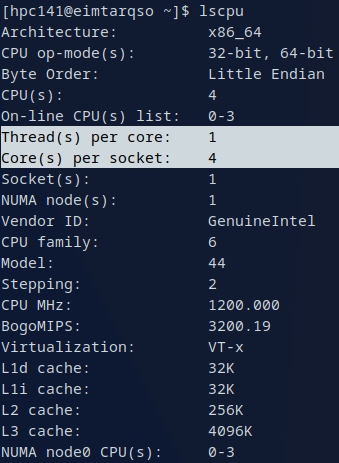
\includegraphics{1.png}
    \caption{lscpu}
    \label{fig:1}
\end{figure}

So, in our cluster we can use up to 4 OpenMP threads.\\

The number of OpenMP threads a user can use in a cluster depends on several factors, including the number of cores and memory available on the nodes, the specific configuration of the cluster and the workload of other users on the system.\\

Inconvenients of using a different configuration for the threads in a cluster for OpenMP:

 \begin{itemize}
  \item Scheduling: Trying to use more threads than allowed by the job scheduler may lead in a job to be queued or rejected.
 \item Performance: Using a different number of threads than the number of available cores can lead overutilization or underutilization of system resources, which can cause performance issues and may even lead to system instability.
 \item Memory usage: Each OpenMP thread requires some amount of memory to operate, so using too many threads can lead to excessive memory usage.
 \end{itemize}

\hypertarget{2}{%
\section{Provide a parallel implementation (OpenMP) of the sum of the different
elements stored in a vector “a” (sum=a[0]+...+a[N-1]) using the reduction clause.}\label{2}}

\begin{lstlisting}[language=C]
 #pragma omp parallel
{
    #pragma omp for
        for(i=0; i<N; i++){
            c[i] = b[i]+a[i];
        }
}

##(we will target this second way in the subsequent examples)
#pragma omp parallel for
    for(i=0; i<N; i++){
        c[i] = b[i]+a[i];
    }
\end{lstlisting}

We can make use of the sum clause suming all elements in a like this:
\begin{lstlisting}[language=C]
  // Calculate the sum of elements stored in the vector "a" in parallel
  #pragma omp parallel for reduction(+:sum)
  for(i=0; i<N; i++){
    sum += a[i];
  }
  \end{lstlisting}

  \textit{*Supposing 'a' has been initialized.}

\hypertarget{3}{%
\section{Provide a parallel implementation (OpenMP) of the two versions (mm.c and mm2.c)
and provide the results obtained from executing them using from one (1) to four (4) threads.
You are requested to follow methodology used in the first assignment (i.e., automating multiple
executions providing statistical results).}\label{3}}

Parallel implementations:

\begin{lstlisting}[language=C, caption=pmm.c: Parametrization of mm.c]
#include <stdlib.h>
#include <stdio.h>
#include <unistd.h>
#include <errno.h>
#include <sys/types.h>
#include <memory.h>
#include <malloc.h>
#include <omp.h>

#define SIZE 1000

int main(int argc, char **argv) {

  float matrixa[SIZE][SIZE], matrixb[SIZE][SIZE], mresult[SIZE][SIZE];
  int i,j,k;

  /* Initialize the Matrix arrays */
  #pragma omp parallel for private(i, j)
  for (i = 0; i < SIZE; i++) {
    for (j = 0; j < SIZE; j++) {
      mresult[i][j] = 0.0;
      matrixa[i][j] = matrixb[i][j] = rand()*(float)1.1;
    }
  }

  /* Matrix-Matrix multiply */
  #pragma omp parallel for private(i, j, k) shared(matrixa, matrixb, mresult)
  for (i = 0; i < SIZE; i++) {
    for (j = 0; j < SIZE; j++) {
      for (k = 0; k < SIZE; k++) {
        mresult[i][j] += matrixa[i][k] * matrixb[k][j];
      }
    }
  }

  exit(0);
}

\end{lstlisting}

\begin{lstlisting}[language=C,caption=pmm2.c: Parametrization of mm2.c]
#include <stdlib.h>
#include <stdio.h>
#include <unistd.h>
#include <errno.h>
#include <sys/types.h>
#include <memory.h>
#include <malloc.h>
#include <omp.h>

#define SIZE 1000

int main(int argc, char **argv) {

  float matrixa[SIZE][SIZE], matrixb[SIZE][SIZE], mresult[SIZE][SIZE];
  int i,j,k;

  /* Initialize the Matrix arrays */
  #pragma omp parallel for collapse(2)
  for ( i=0; i<SIZE; i++ ){
    for ( j=0; j<SIZE; j++ ){
      mresult[i][j] = 0.0;
      matrixa[i][j] = matrixb[i][j] = rand()*(float)1.1;
    }
  }

  /* Matrix-Matrix multiply */
  #pragma omp parallel for private(k, i, j)
  for (k=0;k<SIZE;k++){
   for(j=0;j<SIZE;j++){
    for(i=0;i<SIZE;i++){
      mresult[i][j]=mresult[i][j] + matrixa[i][k]*matrixb[k][j];
    }
   }
  }

  exit(0);
}
\end{lstlisting}

Alongside, we developed the next scripts:

\begin{lstlisting}[language=bash,caption=pmm.sge: SGE template file]
#!/bin/bash
#$ -cwd
#$ -S /bin/bash
#$ -N pmmVERSION_THREADS
#$ -o pmmVERSION_THREADS.out.$JOB_ID
#$ -e pmmVERSION_THREADS.out.$JOB_ID
#$ -pe openmp THREADS

time ./pmmVERSION
\end{lstlisting}

\begin{lstlisting}[language=bash,caption=run.sh: Helper script]
#!/bin/sh

for v in {1,2}; do
for i in {1,2,3,4}; do
	export OMP_NUM_THREADS=$i;
	cp pmm.sge pmm$i.sge;
	sed -i 's/THREADS/'$i'/g' pmm$i.sge
	sed -i 's/VERSION/'$v'/g' pmm$i.sge
	qsub pmm$i.sge
done;
done;
\end{lstlisting}

Each parametrization of mm is called pmm1 or pmm2, depending on the version of mm. pmm.sge contains two sentinel words to change with sed: VERSION and THREAD. VERSION refers to either 1 or 2 in pmm1 and pmm2. THREADS is the number of threads OpenMP will use, from 1 to 4.
run.sh is a script that will generate each SGE iterating over versions and number of threads. For each version of the file will export the number of threads, will make changes in pmm.sge file and send the file to the queue. After some scripting we can do some statistical results with Python:

\begin{figure}[h!]
    \centering
    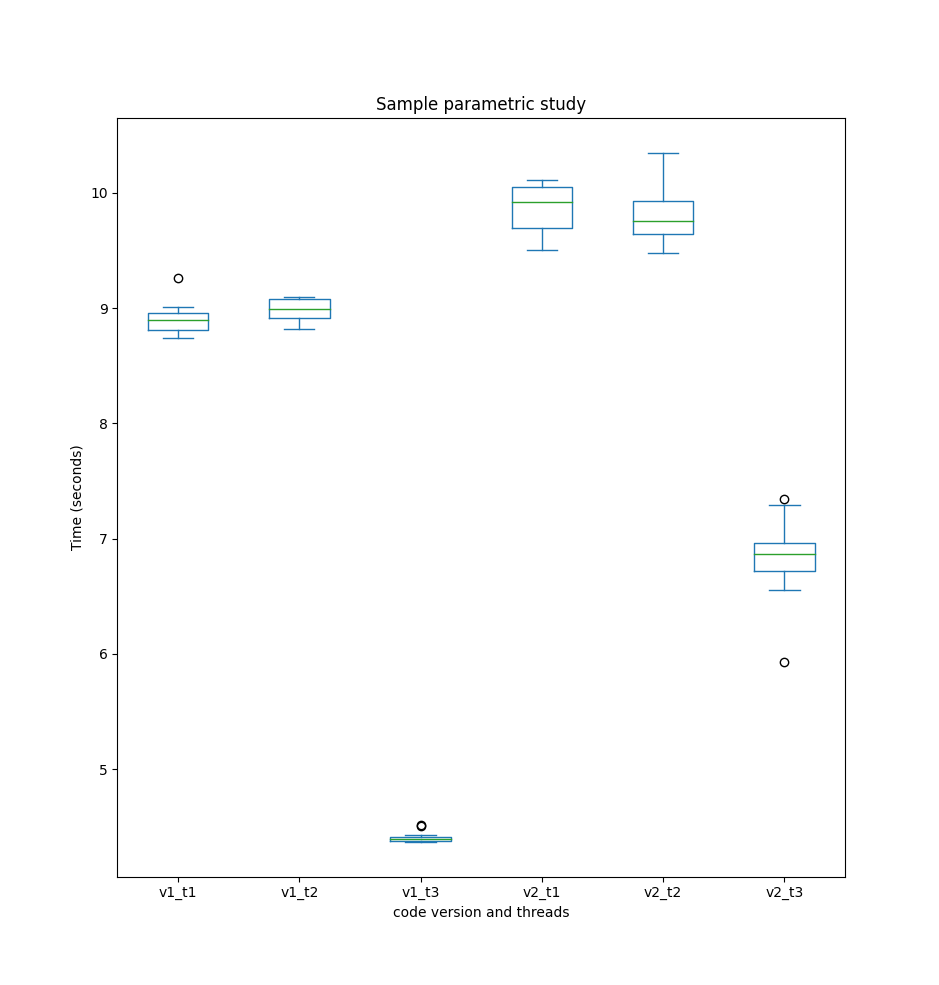
\includegraphics{2.png}
    \caption{Statistic analysis}
    \label{fig:1}
\end{figure}

\begin{lstlisting}[language=Python]
import pandas as pd

from matplotlib import pyplot as plt
from os import walk

data = {}
# get data from results files
for dirpath, dirnames, filenames in walk("."):
    for filename in filenames:
        if not filename.endswith(".py"):
            fname, threads = filename.split(".")[0].split("_")
            # values with 4 threads are discarded because they do not provide enough values
            if threads == "4":
                continue
            version = fname.split("pmm")[1]
            key = f"v{version}_t{threads}"
            if not key in data:
                data[key] = []
            with open(filename, "r") as _file:
                content = _file.readlines()
                time = content[1].split("\t")[1].strip().split("m")[1].rstrip("s")
                data[key].append(float(time))

df = pd.DataFrame(data)
df = df.reindex(sorted(data.keys()), axis=1)

p = df.plot.box()
p.set_title("Sample parametric study")
p.set_xlabel("code version and threads")
p.set_ylabel("Time (seconds)")
plt.show()

\end{lstlisting}

\hypertarget{4}{%
\section{Why do you think there is a difference in execution time and MFLOPs?}\label{4}}

\begin{lstlisting}[language=bash, caption=flops execution]
    [hpc141@eimtarqso ~]$ ./flops; ./flops2
Real_time:	11.539018
Proc_time:	11.511601
Total flpins:	2000964624
MFLOPS:		173.821579
flops.c	PASSED
Real_time:	13.255196
Proc_time:	13.223212
Total flpins:	2003602539
MFLOPS:		151.521622
flops2.c	PASSED
\end{lstlisting}

The difference between process time and MFLOPs is due to the fact that they are measuring different aspects of the program's performance.

Process time is the amount of time that the CPU spends executing the program.  MFLOPs, on the other hand, is a measure of the program's floating-point operations per second (FLOPs) normalized to millions of FLOPs per second (MFLOPs). It gives an indication of the speed of the program's arithmetic operations.

The process time measures the total time taken by the program to execute, including any overhead from the operating system. Meanwhile, MFLOPs measures the number of floating-point operations performed per second, so it reflects the efficiency of the algorithm used in the program.

\hypertarget{5}{%
\section{What hardware counters would you use to study the differences between the two
implementations? Why?}\label{5}}

IPC measures the number of instructions that can be executed per cycle, indicating how well a CPU can utilize its resources to execute instructions. High IPC values suggest that a CPU is executing instructions efficiently, whereas low IPC values may indicate that there are instruction dependencies, pipeline stalls, or cache misses, all of which can negatively impact performance.

Cache misses are a common cause of reduced IPC and code inefficiency. When the CPU tries to access data that is not in the cache, a cache miss occurs. To improve code efficiency, it is important to minimize the number of cache misses.

With PIPA hardware counters we can identify areas of code that may be causing cache misses and reducing IPC. By analyzing hardware performance counters related to cache behavior, PIPA can identify the specific types of cache misses that are occurring, such as L1 or L2 cache misses. This information can then be used to optimize the code by reducing the number of cache misses and improving IPC.

In our case, L2 cache hardware counters are not available, we make use of the next counters:

\begin{itemize}
    \item $PAPI\_TOT\_INS$: Instructions completed
    \item $PAPI\_FP\_OPS$: Floating point operations
    \item $PAPI\_L1\_DCM$: Level 1 data cache misses
    \item $PAPI\_L1\_ICM$: Level 1 instruction cache misses
\end{itemize}

Level 1 (L1) cache misses are the misses that occur in the primary cache, typically the smallest and fastest cache in the system. These misses are often the fastest to resolve since they are the first level of cache accessed by the processor.

\hypertarget{6}{%
\section{Provide the code where you use hardware counters to quantify the differences
between the two examples. Provide the results obtained.}\label{6}}
With the provided examples of matrix multiplication we can make a study on how changing the loops may impact its overall performance, hereby is the code provided adding those PIPA counters:

\begin{lstlisting}[language=C, caption=papi1.c from counters.c]
#include <stdlib.h>
#include <stdio.h>
#include <unistd.h>
#include <errno.h>
#include <sys/types.h>
#include <memory.h>
#include <malloc.h>
#include <papi.h>

#define SIZE 1000
#define NUM_EVENTS 4

int main(int argc, char **argv) {

  float matrixa[SIZE][SIZE], matrixb[SIZE][SIZE], mresult[SIZE][SIZE];
  int i,j,k;
  int events[NUM_EVENTS] = {PAPI_TOT_INS, PAPI_FP_OPS, PAPI_L1_DCM, PAPI_L1_ICM }, ret;
  long long values[NUM_EVENTS];

  if (PAPI_num_counters() < NUM_EVENTS) {
  	fprintf(stderr, "No hardware counters here, or PAPI not supported.\n");
  	exit(1);
  }

  if ((ret = PAPI_start_counters(events, NUM_EVENTS)) != PAPI_OK) {
  	fprintf(stderr, "PAPI failed to start counters: %s\n", PAPI_strerror(ret));
  	exit(1);
  }

  /* Initialize the Matrix arrays */
  for ( i=0; i<SIZE*SIZE; i++ ){
    mresult[0][i] = 0.0;
    matrixa[0][i] = matrixb[0][i] = rand()*(float)1.1; }

  /* Matrix-Matrix multiply */
  for (i=0;i<SIZE;i++)
   for(j=0;j<SIZE;j++)
    for(k=0;k<SIZE;k++)
      mresult[i][j]=mresult[i][j] + matrixa[i][k]*matrixb[k][j];

  if ((ret = PAPI_read_counters(values, NUM_EVENTS)) != PAPI_OK) {
  	fprintf(stderr, "PAPI failed to read counters: %s\n", PAPI_strerror(ret));
  	exit(1);
  }

  printf("Total instructions: %lld\n", values[0]);
  printf("Total hardware flops: %lld\n",values[1]);
  printf("Total L1 data cache misses: %lld\n", values[2]);
  printf("Total L1 instruction cache misses: %lld\n", values[3]);

  exit(0);
}

\end{lstlisting}

\begin{lstlisting}[language=C, caption=papi2.c from counters2.c]
#include <stdlib.h>
#include <stdio.h>
#include <unistd.h>
#include <errno.h>
#include <sys/types.h>
#include <memory.h>
#include <malloc.h>
#include <papi.h>

#define SIZE 1000
#define NUM_EVENTS 4

int main(int argc, char **argv) {

  float matrixa[SIZE][SIZE], matrixb[SIZE][SIZE], mresult[SIZE][SIZE];
  int i,j,k;
  int events[NUM_EVENTS] = {PAPI_TOT_INS, PAPI_FP_OPS, PAPI_L1_DCM, PAPI_L1_ICM}, ret;
  long long values[NUM_EVENTS];

  if (PAPI_num_counters() < NUM_EVENTS) {
  	fprintf(stderr, "No hardware counters here, or PAPI not supported.\n");
  	exit(1);
  }

  if ((ret = PAPI_start_counters(events, NUM_EVENTS)) != PAPI_OK) {
  	fprintf(stderr, "PAPI failed to start counters: %s\n", PAPI_strerror(ret));
  	exit(1);
  }

  /* Initialize the Matrix arrays */
  for ( i=0; i<SIZE*SIZE; i++ ){
    mresult[0][i] = 0.0;
    matrixa[0][i] = matrixb[0][i] = rand()*(float)1.1; }

  /* Matrix-Matrix multiply */
  for (k=0;k<SIZE;k++)
   for(j=0;j<SIZE;j++)
    for(i=0;i<SIZE;i++)
      mresult[i][j]=mresult[i][j] + matrixa[i][k]*matrixb[k][j];

  if ((ret = PAPI_read_counters(values, NUM_EVENTS)) != PAPI_OK) {
  	fprintf(stderr, "PAPI failed to read counters: %s\n", PAPI_strerror(ret));
  	exit(1);
  }

  printf("Total instructions: %lld\n", values[0]);
  printf("Total hardware flops: %lld\n",values[1]);
  printf("Total L1 data cache misses: %lld\n", values[2]);
  printf("Total L1 instruction cache misses: %lld\n", values[3]);

  exit(0);
}

\end{lstlisting}

\begin{figure}[h!]
    \centering
    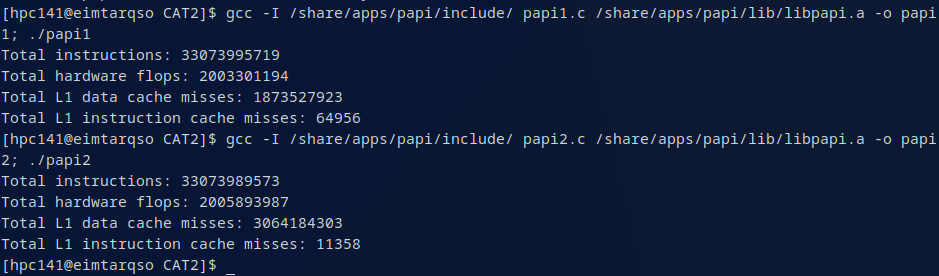
\includegraphics{papi.png}
    \caption{PAPI analysis}
    \label{fig:papi}
\end{figure}

\begin{table}[]
\begin{tabular}{|r|c|c|c|}
\hline
  &  \textbf{papi1} & \textbf{papi2}  \\ \hline
 \textbf{Total Instructions} &  33073995719 & 33073989573   \\ \hline
\textbf{Total hardware flops} &  2003301194 & 2005893987  \\ \hline
 \textbf{L1 data cache misses} & 1873527923 & 3064184303  \\ \hline
 \textbf{L1 instruction cache misses} & 64956 & 11358  \\ \hline
\end{tabular}
\caption{papi1 and papi2 executions}
\label{tab:papi_exec}
\end{table}

papi2 made 6140 less total instructions but 2592793 more hardware flops than papi1. papi2 has over 1190656380 data cache misses than papi1 but has 53598 instruction cache misses less than papi1.


\hypertarget{7}{%
\section{ Provide the requested performance study in terms of execution time and speedup.}\label{7}}

We developed two scripts for this exercise. One that deals with the execution of the SGE file and a SGE file template. The first script will be run 10 times to gather the results of the benchmarks.

\begin{lstlisting}[language=bash,caption=nasa.sge: NPB SGE template file]
#!/bin/bash
#$ -cwd
#$ -S /bin/bash
#$ -N nasa_BENCHMARK_SIZE_THREADS
#$ -o nasa_BENCHMARK_SIZE_THREADS.out.$JOB_ID
#$ -e nasa_BENCHMARK_SIZE_THREADS.out.$JOB_ID
#$ -pe openmp THREADS

/home/hpc141/CAT2/NPB3.2-OMP/bin/BENCHMARK.SIZE
\end{lstlisting}

\begin{lstlisting}[language=bash,caption=nasa.sh: Helper script]
#!/bin/sh

for benchmark in {ft,sp,lu}; do
for size in {w,a}; do
for threads in {1,2,3,4}; do
	export OMP_NUM_THREADS=$i;
	sge=nasa$benchmark_$size_$threads.sge;
	cp nasa.sge $sge
	sed -i 's/THREADS/'$threads'/g' $sge
	sed -i 's/BENCHMARK/'$benchmark'/g' $sge
	sed -i 's/SIZE/'$size'/g' $sge
	qsub $sge
done;
done;
done;
\end{lstlisting}

nasa.sh is a script that will generate each SGE iterating over benchmark, sizes and number of threads.

After 10 executions we have enough to make a study in terms of execution and speedup with Python:

\begin{lstlisting}[language=Python,caption=Python helper script]
import pandas as pd

from matplotlib import pyplot as plt
from os import walk

data = {}
# get data from results files
for _, dirnames, _ in walk("."):
    for _dir in dirnames:
        for _, _, filenames in walk(_dir):
            for filename in filenames:
                if not filename.endswith(".sge"):
                    _, benchmark, size, trail = filename.split("_")
                    threads = trail.split(".")[0]
                    key = f"{benchmark}.{size}-{threads}"
                    if not key in data:
                        data[key] = []
                    with open(f"{_dir}/{filename}", "r") as _file:
                        content = _file.readlines()
                    # find our time in seconds
                    t_in_seconds_str = [t for t in content if t.strip().startswith("Time in seconds")]
                    t_in_seconds = float(t_in_seconds_str[0].strip().split("=")[-1])
                    data[key].append(float(t_in_seconds))

df = pd.DataFrame(data)
df = df.reindex(sorted(data.keys()), axis=1)

p = df.plot.box()
p.set_title("Performance study")
p.set_xlabel("Benchmark version and threads")
p.set_ylabel("Time (seconds)")
plt.show()

\end{lstlisting}

\begin{figure}[ht]    
    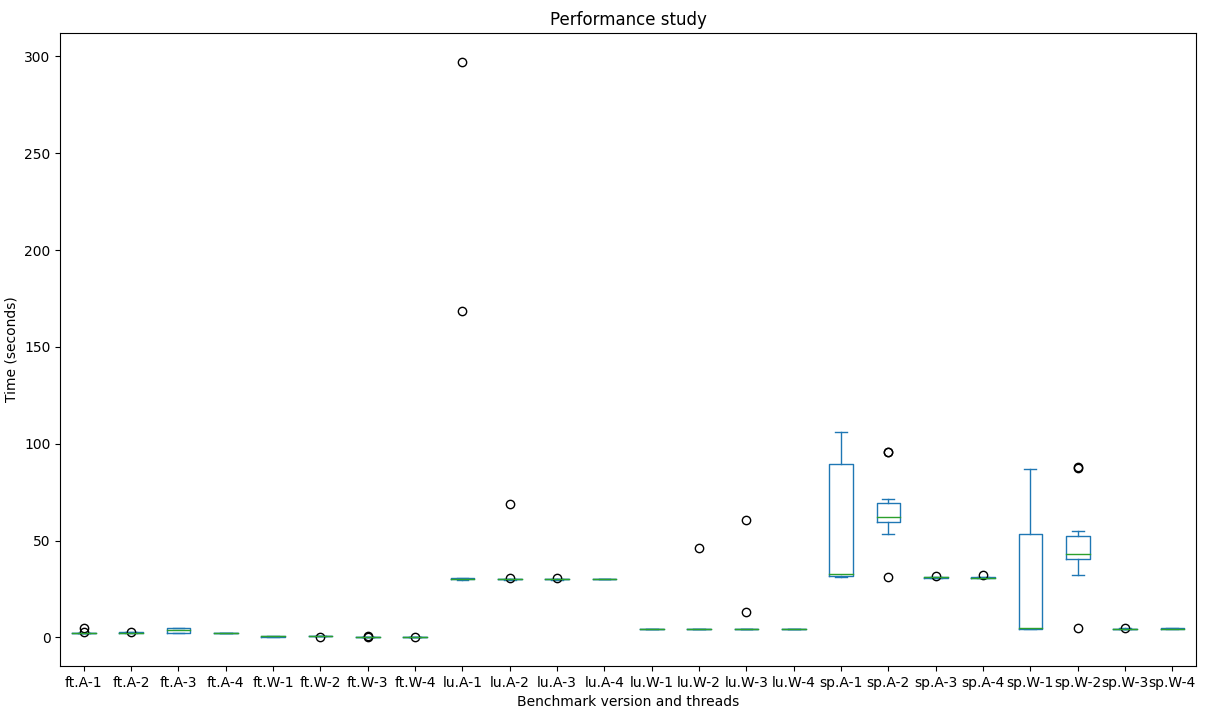
\includegraphics{performance.png}
    \caption{Performance study}
    \label{fig:nasa}
\end{figure}

\hypertarget{9}{%
\section{Provide a parallel implementation (OpenMP) of the sequential program in q9.c. You
can make code transformations as long as they do not modify the program functionality. Provide
your design decisions to improve performance/balance and performance evaluation.}\label{9}}

\begin{lstlisting}[language=C]
#include <stdlib.h>
#include <stdio.h>
#include <time.h>
#include <omp.h>

#define N 16000
#define T 4

int main(int argc, char **argv) {

  long long A[T][N], B[T][N], avg[T];
  int i,j,k,l,sum,elems;

  srand(time(NULL));

  #pragma omp parallel for private(j)
  for(i=0; i<T; i++){
   for(j=0; j<N; j++){
    if(i<T/2){
     A[i][j]=N/2+rand()%(N/2);
    }
    else{
     A[i][j]=rand()%(N/8); 
    }
   }
  }

  #pragma omp parallel for private(j,k,l,sum)
  for(i=0; i<T; i++){
   for(j=0; j<N; j++){
    sum=0;
    for(k=0; k<A[i][j]; k++){
     for(l=0; l<T; l++){
      if(l!=i){
       sum=(sum+A[l][j])%(N/8);
      }
     }
    }
    B[i][j]=(A[i][j]+sum)%N;
   }
  }

  #pragma omp parallel for private(j,k,l,sum) shared(avg)
  for(i=0; i<2; i++){
   elems=N/2+rand()%(N/4);
   sum=0;
   for(j=0; j<N; j++){
     for(k=0; k<A[i][j]; k++){
       for(l=0; l<T; l++){
         sum=(sum+A[l][j])%(N/4);
       }
     }
   }
   avg[i]=sum/elems;
  }

  #pragma omp parallel for private(j)
  for(i=0; i<T; i++){
   for(j=0; j<N; j++){
     B[i][j]+=A[i][j]+avg[1];
   }
  }

  exit(0);
}
\end{lstlisting}

We use the "private" clause to ensure that each thread has its own copy of the loop index variables and shared clauses to ensure that the threads do not interfere with each other's data. We have also added OpenMP directives to parallelize the outer loops.

\cite{texbook}

\bibliographystyle{abbrvnat}
\bibliography{bibliography}

\end{document}
